\documentclass{beamer}
\usetheme{Zurich}
\usepackage{amsmath, amsfonts, graphicx, multirow}
\title{Random Forests}
\author{Charlotte Wickham}
\date{\today}

\begin{document}

\frame{\titlepage}

\begin{frame}
	\frametitle{Random Forests}
\begin{definition}	
	A random forest is a classifier consisting of a collection of tree-structured classifiers $\{h (x, \Theta_k ), k = 1, \ldots\}$ where the $\{\Theta_k \}$ are independent identically distributed 
random vectors and each tree casts a unit vote for the most popular class at input x.
\end{definition}
\begin{itemize}
	\item Bagging is one example.  Here the $\Theta_i$ is vector representing a bootstrap sample from the training set.
	\item Another example is random split selection (to be discussed later).  Here $\Theta_i$ is a vector of random integers indexing the input to be split on at each node.
\end{itemize}
	
The nature and dimension of $\Theta_k$	depends on its use in the tree construction process.
\end{frame}

\begin{frame}
	\frametitle{Why do random forests work?}
	\begin{itemize}
		\item Weak learners have low bias but high variance.
		\item Averaging weak learners, over many training sets, gives estimates with low bias and low variance.
		
	\end{itemize}

\end{frame}

\begin{frame}
	\frametitle{Why do random forests work?}
	Let the margin of the random forest be,
	\[
	mr(X,Y) = P_\Theta(h(X,\Theta) = Y) - \max_{j\ne Y}P_\Theta (h(X,\Theta) = j).
	\]
	And define the strength of the set of classifiers ${h(X,\Theta)}$ to be,
	\[
	s = E_{X,Y}mr(X,Y).
	\]
	
	Also define, 
	\[
	\bar{\rho} = E_{\Theta, \Theta'}(\rho(\Theta, \Theta')sd(\Theta)sd(\Theta'))/ E_{\Theta, \Theta'}(sd(\Theta)sd(\Theta')),
	\]	
	to be the mean value of the correlation  between trees.

\end{frame}

\begin{frame}
	\frametitle{Why do random forests work?}
	Can show that the generalization error of the forest, $PE^*$ is bounded above by,
	\[
	PE^* \le \bar{\rho}(1-s^2)/s^2.
	\]
	
	So, for low error we want high strength and low correlation.
	
	\begin{itemize}
		\item High Strength
			\begin{itemize}
				\item Grow tree to maximum depth
			\end{itemize}
		\item Low correlation
		\begin{itemize}
			\item Grow each tree from a bootstrap sample
			\item Add some other form of randomness 
		\end{itemize}
	\end{itemize}
	
\end{frame}

\begin{frame}[fragile]
	\frametitle{Random input selection}
	Fix parameter $K$
	\begin{itemize}
		\item Draw a bootstrap sample from the training set
		\item Grow full size tree as usual except at each node choose $K$ variables randomly on which to search for the best split.
		\item Repeat $N$ times to generate $N$ trees.
	\end{itemize}
	Breiman suggests $K=\sqrt{\text{number of variables}}$.

	Implemented in R in \verb|randomForest| .
	
\end{frame}

\begin{frame}
	\frametitle{Random linear combination of variables}
	Fix parameters $L$ and $F$
	\begin{itemize}
		\item Draw a bootstrap sample from the training set
		\item Choose $L$ variables randomly and combine them using coefficients drawn uniformly on $[-1,1]$. Create $F$ of these linear combinations and search for which gives the best split.
		\item Repeat $N$ times to generate $N$ trees.
	\end{itemize}
	Should standardize variables first.
	Some problems with categorical variables
	\begin{itemize}
		\item Transform to a dummy variable by picking a random selection of levels to be 1.
		\item Let categorical variables be $I-1$ times as likely to be picked as continuous variables.
	\end{itemize}
	Not implemented in R.
\end{frame}

\begin{frame}
	\frametitle{Out of bag estimates.}
	For each tree in the forest we can use the observations that were not in the bootstrap sample to estimate measures of interest.
	
	\item{Misclassification rate}
	\begin{itemize}
		\item 		For each tree find the classification for the out of bag observations
		\item 		Classification of a point is the plurality in classification over all trees in which an observation was out of bag 
		\item 		Use classification to calculate error rate
	\end{itemize}
		
\end{frame}

\begin{frame}
	\frametitle{Exploring the Random Forest mechanism.}
	Results in a black box.  How can we investigate the structure of the data.
	\begin{itemize}
		\item Variable Importance
			\begin{itemize}
				\item Use out of bag observations and randomly permute one variable.  
				\item Run the observations down the tree and record classification.
				\item Repeat for each tree.
				\item Compare the misclassification rate with the noised up variable to the out of bag estimate without permutation.
				\item Variable Importance = percent increase in misclassification.
			\end{itemize}
		\item Proximity
		\begin{itemize}
			\item Proximity between observations $i$ and $j$ is the proportion of trees in which the observations occur together in a terminal node.
		\end{itemize}
	\end{itemize}
\end{frame}


\begin{frame}[fragile]
	\frametite{Supernova Data}
	\begin{small}
	\begin{verbatim}
	Call:
	 randomForest(formula = class ~ ., data = nova.train,
	 	importance = TRUE, proximity = TRUE, keep.forest = FALSE,
	 	ntree = 1000) 
	
	               Type of random forest: classification
	                     Number of trees: 1000
	No. of variables tried at each split: 4

	        OOB estimate of  error rate: 4.2%
	Confusion matrix:
	      Other   SN class.error
	Other  4386  114  0.02533333
	SN      264 4236  0.05866667
	\end{verbatim}
	\end{small}
\end{frame}

\begin{frame}
	\frametitle{Preformance on test set}
	\begin{table}
	\begin{tabular}{cr|rr}
	& & \multicolumn{2}{c}{Prediction}\\
	& & Other & Supernova\\
	\hline
	\multirow{2}{*}{\rotatebox{90}{Actual}} & Other &  484 &  16\\
	& Supernova & 39 &  461\\
	\end{tabular}
	\end{table}
	Error: 5.5\%
	
	(were getting about 8\% from CART and 6\% from bagging.)
\end{frame}

\begin{frame}
	\frametitle{Supernova - Variable Importance}
	\setkeys{Gin}{width = \textwidth}
	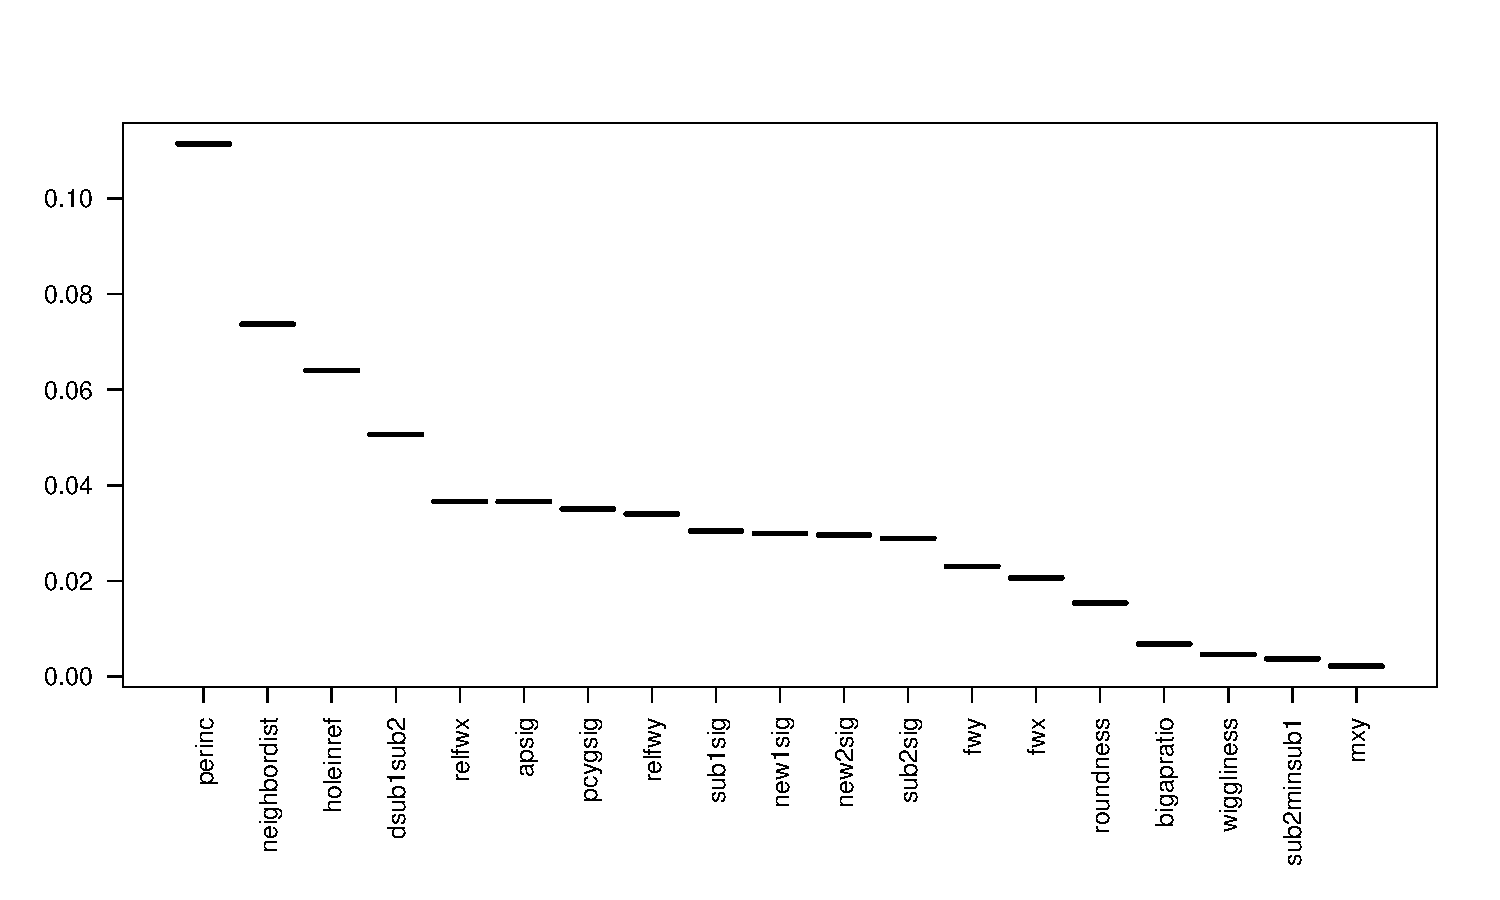
\includegraphics{imp.pdf}
\end{frame}

\begin{frame}[fragile]
	\frametitle{Supernova Data - Try different K}
	\begin{itemize}
		\item K = 2
		\begin{table}
		\begin{tabular}{cr|rr}
		& & \multicolumn{2}{c}{Prediction}\\
		& & Other & Supernova\\
		\hline
		\multirow{2}{*}{\rotatebox{90}{Actual}} & Other &  484 &  16\\
		& Supernova & 38 &  462\\
		\end{tabular}
		\end{table}
		Error: 5.4\%
		
		\item K = 8
		\begin{table}
		\begin{tabular}{cr|rr}
		& & \multicolumn{2}{c}{Prediction}\\
		& & Other & Supernova\\
		\hline
		\multirow{2}{*}{\rotatebox{90}{Actual}} & Other &  480 &  20\\
		& Supernova & 37 &  463\\
		\end{tabular}
		\end{table}
		Error: 5.7\%
	\end{itemize}
\end{frame}

\end{document}